\documentclass[12pt,a4paper]{report}

\usepackage[utf8]{inputenc}
\usepackage[english]{babel}
\usepackage{amsmath}
\usepackage{amsfonts}
\usepackage{amssymb}
\usepackage{graphicx}
\usepackage{cite}
\usepackage[left=2cm,right=2cm,top=2cm,bottom=2cm]{geometry}

\author{Josep Maria Serra Moncunill}
\title{Satellite Frequencies}


\begin{document}
\maketitle

\chapter{Frequencies}

\section{Frequency spectre}
\paragraph{}Satellite communications are done using electromactetic waves which are part of the Radio Frequency (RF) spectrum. This spectrum covers from 3Hz to 3000Ghz. Acording to the International Telecommunication Union, the RF spectrumis divided in 12 bands, equally distributed in a logaritmic scale. In this range of frequencies, the most used ones, including satellite communication frequencies, are subdivided into subbands. This subdivisions are diferent according to the Institute of Electrical and Electronics Engineers (IEEE) classification or the NATO classification.\\
\\
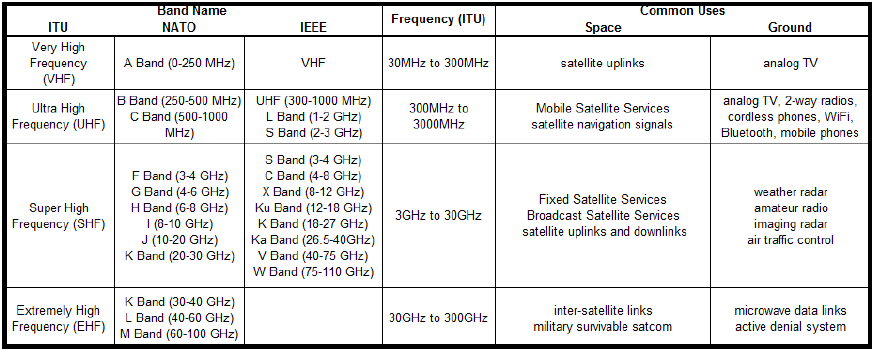
\includegraphics[scale=0.75]{spectrum.png}

\paragraph{}It is important to take into account that, for ground-to-satellite communications, frequencies under 30MHz are absorbed by the ionosphere. The same occurs with frequencies over 30GHz, which are absorbed by oxygen and water vapour (rain fade). Therefore, satellite communications between ground and space must take place in the 30Mhz-30GHz range.

\paragraph{}The following list contains the most used frequencies for satellite communications in each of the diferend bands.

\begin{itemize}
\item VHF Band
	\begin{itemize}
	\item \textbf{136-138 MHz}\\
	This band was used heavily by many different types of satellites in the past. Today (2012), most activity is restricted to 137-138 MHz (which is the current allocation) and consists of meteorological satellites transmitting data and low resolution images, together with low data rate mobile satellite downlinks (eg Orbcomm)
	\item \textbf{144-146 MHz}\\
	One of the most popular bands for amateur satellite activity. Most of the links are found in the upper half of the band (145-146 MHz).
	\item \textbf{148-150 MHz}\\
	This tends to be used for uplinks of the satellites that downlink in the 137 - 138 MHz band.
	\item \textbf{149.95-150.05 MHz}\\
	This is used by satellites providing positioning, time and frequency services, by ionospheric research and other satellites. Before the advent of GPS it was home to large constellations of US and Russian satellites that provided positioning information (mainly to marine vessels) by use of the Doppler effect). Many satellites transmitting on this band also transmit a signal on 400 MHz.
	\item \textbf{240-270 MHz}\\
	Military satellites, communications. This band lies in the wider frequency allocation (225-380 MHz) assigned for military aviation.
	\end{itemize}
\item UHF Band
	\begin{itemize}
	\item \textbf{399.9-403 MHz}\\
	This band includes navigation, positioning, time and frequency standard, mobile communication, and meteorological satellites. Around 400 MHz is a companion band for satellites transmitting on 150 MHz.
	\item \textbf{432-438 MHz}\\
	This range includes a popular amateur satellite band as well as a few Earth resources satellites.
	\item \textbf{460-470 MHz}\\
	Meteorological and environmental satellites, includes uplink frequencies for remote environmental data sensors.
	\end{itemize}
\item L Band
	\begin{itemize}
	\item \textbf{1.2-1.8 GHz}
	\\This frequency range includes a very diverse range of satellites and encompasses many sub-allocations. This range includes the GPS and other GNSS (Global Navigation Satellite Systems - Russian Glonass, European Galileo, Chinese Beidou). It also hosts SARSAT/COSPAS search and rescue satellites which are carried on board US and Russian meteorological satellites. It also includes a mobile satellite communication band.
	\item \textbf{1.67-1.71 GHz}
	\\This is one of the primary bands for high resolution meteorological satellite downlinks of data and imagery.
	\end{itemize}
\item S Band
	\begin{itemize}
	\item \textbf{2.025-2.3 GHz}\\
	Space operations and research, including 'deep space' links from beyond Earth orbit. This encompasses the Unified S-band (USB) plan which is used by many spacecraft, and which was also used by the Apollo lunar missions. It also includes military space links including the US Defense Meteorological Satellite Program (DMSP). Many Earth resources (remote sensing) satellites downlink in this band.
	\item \textbf{2.5-2.67 GHz}\\
	Fixed (point-to-point) communication and broadcast satellites, although the broadcast allocation is only used in some Asian and Middle-eastern countries.
	\end{itemize}
\item C Band
	\begin{itemize}
	\item \textbf{3.4-4.2 GHz}\\
	Fixed satellite service (FSS) and broadcast satellite service (BSS) downlinks. International TV broadcast uses this allocation heavily.
	\item \textbf{5.9-6.4 GHz}\\
	This is the FSS/BSS uplink for the 3.4-4.2 GHz downlink band.
	\end{itemize}
\item X Band
	\begin{itemize}
	\item \textbf{8-9 GHz}\\
	This is used heavily for space research, deep space operations, environmental and military communication satellites. Many satellites/spacecraft carry complementary S and X band transmitters.
	\end{itemize}
\item Ku Band
	\begin{itemize}
	\item \textbf{10.7-11.7 GHz}\\
	Fixed satellite services (FSS)
	\item \textbf{11.7-12.2 GHz}\\
	Broadcast satellite service (BSS) downlinks. This band is used for domestic TV programs.
	\item \textbf{14.5-14.8 GHz}\\
	The uplink for the previous Ku downlink band.
	\item \textbf{17.3-18.1} GHz\\
	An alternate 'Ku' band BSS uplink.
	\end{itemize}
\item Ka Band
	\begin{itemize}
	\item \textbf{23-27 GHz}\\
	A region that will be used increasingly by a variety of fixed link, broadcast, environmental and space operations satellites in the future as more bandwidth is required than can be provided in the lower bands. The disadvantage of this band is the increased absorption due to water vapour and rain. Not very useful for tropical regions of the Earth.
	\end{itemize}
\end{itemize}

\section{Regulation}
\paragraph{}The ITU is the organization that regulates the utilization of radio frequencies.  The ITU Radio Regulations comprise and regulate the part of the allocated radio frequency spectrum from 9 kHz to 275 GHz. According to ITU-RR, the world is divided into 3 regions, and allocation of radio frequencies can be different in those regions. Region 1 comprises Europe, Africa and the northern part of Asia; Region 2 is Northern America, South America and Greenland; Region 3 is the rest of Asia and Oceania.

\paragraph{}The ITU Radio Regulations define: the allocation of different frequency bands to different radio services; the mandatory technical parameters to be observed by radio stations, especially transmitters; procedures for the coordination (ensuring technical compatibility) and notification (formal recording and protection in the Master International Frequency Register) of frequency assignments made to radio stations by national governments; other procedures and operational provisions. To avoid interfference between frequencies, the ITU Radio Regulations usually allocate similar servicies to the same bandwith, such as TV-Broadcast Geoestationary satellites.

\paragraph{}It is the government of a country the one that delivers a company or a specific collective a license allowing them to transmit in a specific frequency, all of this following the ITU Radio Regulations and the ITU Recomendations. However, for stations that not transmit the license is not required to operate.

\end{document}
